\documentclass[12pt, twoside]{article}
\usepackage[letterpaper, margin=1in, headsep=0.2in]{geometry}
\setlength{\headheight}{0.6in}
%\usepackage[english]{babel}
\usepackage[utf8]{inputenc}
\usepackage{microtype}
\usepackage{amsmath}
\usepackage{amssymb}
%\usepackage{amsfonts}
\usepackage{siunitx} %units in math. eg 20\milli\meter
\usepackage{yhmath} % for arcs, overparenth command
\usepackage{tikz} %graphics
\usetikzlibrary{quotes, angles}
\usepackage{graphicx} %consider setting \graphicspath{{images/}}
\usepackage{parskip} %no paragraph indent
\usepackage{enumitem}
\usepackage{multicol}
\usepackage{venndiagram}

\usepackage{fancyhdr}
\pagestyle{fancy}
\fancyhf{}
\renewcommand{\headrulewidth}{0pt} % disable the underline of the header
\raggedbottom
\hfuzz=2mm %suppresses overfull box warnings

\usepackage{hyperref}

\fancyhead[LE]{\thepage}
\fancyhead[RO]{\thepage \\ Name: \hspace{4cm} \,\\}
\fancyhead[LO]{BECA / Dr. Huson / Geometry\\*  Unit 8: Congruence transformations\\* 6 January 2023}

\begin{document}

\subsubsection*{8.4 Homework: Mixed review \hfill CCSS.HSG.CO.A.5}
\begin{enumerate}
\item Apply a counterclockwise rotation of $90^\circ$ centered at the origin to $\triangle ABC$. Plot and label the image on the axes below and make a table of its coordinates.
\begin{flushright}
  \begin{tikzpicture}[scale=.48]
    \draw [help lines] (-8,-6) grid (8,8);
    \draw [thick, <->] (-8.4,0) -- (8.4,0) node [right] {$x$};
    \draw [thick, <->] (0,-6.4)--(0,8.4) node [above] {$y$};
    \draw [thick]
      (2,1) node[below left] {$A$}--
      (5,5) node[right] {$B$}--
      (6,2) node[below] {$C$}--
      cycle;
  \end{tikzpicture}
\end{flushright}

\item The vertices of $\triangle JKL$ have the coordinates $J(-4,-2)$, $K(-1,-1)$, and $L(-2,3)$, as shown below. \\[0.25cm]
Apply a translation of $(x,y) \rightarrow (x-3, y+2)$ to $\triangle JKL$ and then reflect the image across the $y$-axis. Draw both images $\triangle J'K'L'$ and $\triangle J''K''L''$ on the set of axes below, labeling the vertices.
\begin{flushright}
  \begin{tikzpicture}[scale=.48]
    \draw [help lines] (-8,-8) grid (8,8);
    \draw [thick, <->] (-8.4,0) -- (8.4,0) node [right] {$x$};
    \draw [thick, <->] (0,-8.4)--(0,8.4) node [above] {$y$};
    \draw [thick]
      (-4,-2) node[below left] {$J$}--
      (-1,-1) node[right] {$K$}--
      (-2,3) node[above left] {$L$}--
      cycle;
  \end{tikzpicture}
\end{flushright}

\newpage
\item Find the area of the parallelogram $ABCD$ shown below, with $AB=9.5$ and height $h=7.1$.
\begin{flushright}
\begin{tikzpicture}[scale=0.7]
  \draw [-, thick] (0,0)--(5,0)--(6,3)--(1,3)--cycle;
  \draw [-, dashed] (5,0)--(5,3);
  \draw [fill] (0,0) circle [radius=0.05] node[left]{$A$};
  \draw [fill] (5,0) circle [radius=0.05] node[right]{$B$};
  \draw [fill] (6,3) circle [radius=0.05] node[right]{$C$};
  \draw [fill] (1,3) circle [radius=0.05] node[left]{$D$};
  \node at (4.3, 1.5){$7.1$};
  \node at (2.5, -0.5){9.5};
\end{tikzpicture}
\end{flushright}

\item The measures in degrees of the three angles of a triangle are $3x$, $\frac{1}{2}x+7$, and $5x-65$. Find $x$. \vspace{4cm}

\item  A wooden cutting board is $8 \frac{1}{2}$ inches long, 7 inches wide, and $1 \frac{1}{4}$ inches thick. Find the volume of the box. Show the calculation.
\begin{flushright}
\begin{tikzpicture}[scale=1]
  \draw [-, thick] (0,0)--(7,0)--(7,1)--(0,1)--cycle;
  \draw [-, thick] (0,1)--(0.5,2.5)--(7.5,2.5)--(7,1);
  \draw [-, thick] (7,0)--(7.5,1.5)--(7.5,2.5);
  \node at (7.8, 2){$1 \frac{1}{4}$};
  \node at (3.5, -0.35){$8 \frac{1}{2}$};
  \node at (7.6, 0.8){$7$};
\end{tikzpicture}
\end{flushright} \vspace{3cm}

\item Of two complementary angles, the measure of $\angle A$ is two times that of $\angle B$. Find $m\angle A$.\\[0.25cm]
First write an equation for full credit. \vspace{3.5cm} 

\newpage
\item An angle bisector is shown below, with $\overrightarrow{AC}$ bisecting $\angle BAD$. Given $m\angle BAC = 6x-5$ and $m\angle BAD = 9x+17$, find $m\angle BAD$. (Show check)
\begin{flushright}
\begin{tikzpicture}[scale=0.7, rotate=30]
  \draw [<->, thick] (100:7)node[left]{$B$} 
  --(0,0)node[below]{$A$}
  --(6,0)node[below]{$D$}--(7,0);
  \draw [->, thick] (0,0)--(50:7)node[below right]{$C$};
  %\draw [fill] (0,0) circle [radius=0.05] node[below]{$A$};
  %\draw [fill] (5,0) circle [radius=0.05] node[below]{$B$};
\end{tikzpicture}
\end{flushright} \vspace{3cm}

\item Angles $APC$ and $CPD$ form a linear pair. $m\angle APC = 10x-10$ and $m\angle CPD = 3x-5$. Find $m\angle CPD$. Check your answer for full credit.
\begin{flushright}
  \begin{tikzpicture}[scale=0.8, rotate=-10]
    \draw [->, thick] (0,0)--(35:5);
    \draw [<->, thick] (-5,0)--(6,0);
    \draw [->, thick] (0,0)--(0,3);
    \draw (0,0)++(0.3,0)--++(0,0.3)--+(-0.3,0);
    %\draw [fill] (-1,2.5) circle [radius=0.05] node[left ]{$B$};
    \draw [fill] (35:4) circle [radius=0.05] node[below right]{$C$};
    \draw [fill] (-4,0) circle [radius=0.05] node[below]{$A$};
    \draw [fill] (0,0) circle [radius=0.05] node[below left]{$P$};
    \draw [fill] (0,2) circle [radius=0.05] node[left]{$B$};
    \draw [fill] (4,0) circle [radius=0.05] node[below]{$D$};
  \end{tikzpicture}
  \end{flushright}
  \vspace{5cm}

\newpage
\subsubsection*{Do Not Solve! \\
Model the situation with an equation in terms of $x$.}
\item Given $\overline{ABC}$, with $AB=2x-1$, $BC=3x+7$, and $AC=21$. Find $x$. \vspace{1cm}
\begin{flushright}
  \begin{tikzpicture}
    \draw [-, thick] (0,0) node[below]{$A$}--
    (2,0) node[below]{$B$}--
    (6,0) node[below]{$C$};
    \draw [fill] (0,0) circle [radius=0.05];
    \draw [fill] (2,0) circle [radius=0.05];
    \draw [fill] (6,0) circle [radius=0.05];
  \end{tikzpicture}
  \end{flushright} \vspace{1cm}

\item Given $m\angle 3 = x+35$ and $m\angle 5 = 4x-25$. Find $x$. 
\begin{flushright}
\begin{tikzpicture}
  \draw [<->, thick] (3,2)--(8,2);
  \draw [<->, thick] (2,0)--(7,0);
  \draw [<->, thick] (4,-1)--(5.5,3);
  \node at (4.5,0.3) [left]{$5$};
  \node at (4.5,0.3) [right]{$6$};
  \node at (4.3,-0.3) [left]{$7$};
  \node at (4.3,-0.3) [right]{$8$};
  \node at (5.2,2) [above left]{$1$};
  \node at (5.2,2) [above right]{$2$};
  \node at (5,2) [below left]{$3$};
  \node at (5,2) [below right]{$4$};
\end{tikzpicture}
\end{flushright} \vspace{0.5cm}

\item In the diagram below $m\angle AOB = 6x+5$ and $m\angle COB = 8x+15$. Find $x$. %\vspace{0.25cm}
\begin{flushright}
\begin{tikzpicture}[scale=0.7, rotate=30]
\draw [<->, thick] (-25:5)--(0,0)--(155:5);
\draw [<->, thick] (-5,0)--(5,0);
\draw [->, thick] (0,0)--(0,4);
\draw (0,0)++(0.3,0)--++(0,0.3)--+(-0.3,0);
%\draw [fill] (-1,2.5) circle [radius=0.05] node[left ]{$B$};
\draw [fill] (155:3) circle [radius=0.05] node[below left]{$B$};
\draw [fill] (-4,0) circle [radius=0.05] node[below]{$A$}; 
\draw [fill] (0,0) circle [radius=0.05] node[below]{$O$};
\draw [fill] (0,3) circle [radius=0.05] node[left]{$C$};
\draw [fill] (4,0) circle [radius=0.05] node[below]{$D$};
\draw [fill] (-25:2) circle [radius=0.05] node[below]{$E$};
\end{tikzpicture}
\end{flushright}

\item The point $K$ is the midpoint of $\overline{JL}$, $JK=3x+15$, and $JL=9x+9$. Find $x$.  \vspace{1cm}
\begin{flushright}
  \begin{tikzpicture}
    \draw [-, thick] (0,0) node[below]{$J$}--
    (3,0) node[below]{$K$}--
    (6,0) node[below]{$L$};
    \draw [fill] (0,0) circle [radius=0.05];
    \draw [fill] (3,0) circle [radius=0.05];
    \draw [fill] (6,0) circle [radius=0.05];
  \end{tikzpicture}
  \end{flushright} \vspace{2cm}

\end{enumerate}
\end{document}